% !TEX root = ../thesis-example.tex
%
\chapter{Advanced 3D Ultrasound Visualization}
\label{predicates}


Direct volume visualization techniques such as volume ray casting are today's state-of-the-art algorithms for the visualization of three-dimensional medical images. 
In order to approximate the physics of light transport, most techniques use global transfer functions for the classification step of the classic volume rendering pipeline. 
While they yield impressive results for images from tomographic reconstructions such as computed tomography (CT) or magnetic resonance imaging (MRI), global 1D transfer functions reach their limits when being applied to 3D ultrasound images.
Though they have recently become part of clinical practice due to the advances in today's 3D freehand ultrasound systems, effective and generic visualization tools are still missing for this imaging modality.
This is mainly because several characteristics of B-mode ultrasound (brightness mode ultrasound where pixel intensities relate to the change of acoustic impedance and thus the reflectance of the sound wave) let its volumetric visualization suffer from severe occlusion artifacts as shown in Figure \ref{fig:predicates:occlusion}. 

\begin{figure}[ht]
	\centering
	\subfloat[Standard DVR of carotid ultrasound volume]{
		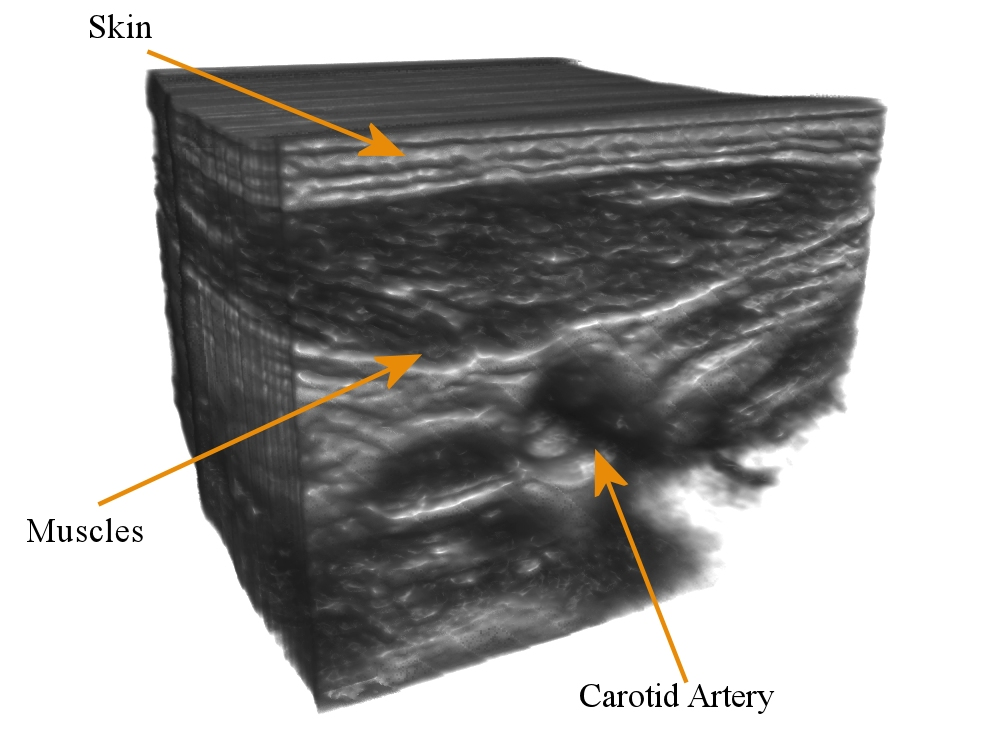
\includegraphics[width=0.75\linewidth]{./figures/predicates/us_dvr_annotated.jpg}
	} \\%
	\subfloat[Intensity distribution and applied TF of the above visualization]{
		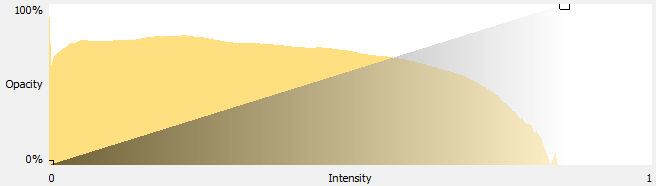
\includegraphics[width=0.75\linewidth]{./figures/predicates/us_dvr_tf.png}
	}	
	\caption{
		\textbf{Occlusion artifacts} of traditional methods:
		(a) While one can see the outer shell of the different layers, clinical relevant information such as the path and shape of the carotid artery and its bifurcation are hidden.
		(b) Due to the homogeneous distribution of ultrasound intensities and their highly context-sensitive nature, there is no chance in discriminating relevant features through their intensities.
	}
	\label{fig:predicates:occlusion}
\end{figure}

In lack of better alternatives, clinicians prefer to look at 2D slices extracted from 3D ultrasound volumes. 
Such multi-planar reconstructions (MPRs) allow for the visualization of arbitrary planes, which is not directly possible with 2D ultrasound. 
However, MPRs are hardly able to expose spatial context and connectivity information to the clinician. 
Rendering extracted geometry from the image obtained by segmentation algorithms, as an alternative, may show connectivity information but does no longer expose the original image data (i.e. ultrasound intensities) and in particular the speckle texture, which is an essential part of ultrasound imaging. 
Therefore, this kind of indirect visualization is not well suited for many clinical routines. 

In order to achieve clinically helpful direct volume visualization, we propose a completely novel approach to the classification stage together with an intuitive tool for setting up the rendering result: We introduce the concept of point predicates, which evaluate both local and global features of the ultrasound image and are defined on every sampling point. 
This facilitates to perform classification also based on high-level non-local information such as speckle or texture or even anatomical models/segmentations. 
By further annotating each predicate with an importance factor, we can naturally implement relevance-based visualization ensuring that important anatomies are always visible in the rendering, while preserving context information where possible in order to show better spatial clues. 

Despite the recent advances regarding quality, interactiveness, and usability, volumetric visualization still has not been fully accepted by most clinicians for their workflow and is, if at all, only used for publications or patient presentations. 
Even with CT imaging, where the image intensities (Hounsfield units) directly correspond to a physical property that allows for direct discrimiation of tissue types, most radiologists still prefer to scroll through the stack of 2D slices and make up the 3D model in their minds instead of looking at 3D visualizations.
This is mainly due to the lack of usability of today's classification approaches, where changing the volume rendering to show different anatomy relates to adaption of the transfer function.
The limited expressiveness and intuitiveness, as well as the high dimensionality of the parameter domain, in particular with multi-dimensional transfer functions, makes their setup a tedious and cumbersome task that many clinicians have difficulties with \cite{Salama06}. 

With this issue in mind, we further introduce the predicate histogram as an effective tool for reducing the dimensionality of the predicate configuration space and facilitating its manipulation. 
Together with the descriptive semantics of predicates, it provides the user with easy and intuitive interaction with the point predicates to setup the rendering. 
This user interface was designed to allow for interactive exploration of clinically relevant information and switching between visualizations of different target anatomies with minimal efforts in a highly intuitive way.
This is further enriched by a scribble technique providing a painting metaphor to specify classification directly in the image domain. 


\section*{Related Work}
\label{sec:predicates:related_work}

Our proposed method has three important properties:
\begin{my_list_num}
	\item It is particularly designed for the visualization of ultrasound volumes. 
	\item It integrates different levels of information, ranging from low-level local image intensities to even anatomical models, into a single consistent formulation that is exposed to the user using an intuitive widget. 
	\item It exploits illustrative focus-and-context rendering techniques. 
\end{my_list_num}

Since the body of literature on volume rendering techniques is large, we focus this section on the most closely related works regarding the above topics and refer the interested reader to the book of Preim and Botha \cite{Preim13} for a more exhaustive overview. 

\subsection{Visualization of Ultrasound Volumes}
\label{sec:predicates:related_work:us}

Compared to tomographic imaging modalities such as CT or MRI, where direct volume rendering can show very distinct visualizations of the anatomy, B-mode ultrasound images provide special challenges to classification causing these techniques to fail in yielding helpful visualizations. 
Since ultrasound imaging exploits the echo generated by density changes at tissue interfaces of different acoustic impedance, it rather shows the changes in physical properties than the physical properties themselves. 
As a consequence, ultrasound images are fundamentally different to those obtained from tomographic imaging modalities. 
In addition to this gradient-like nature, ultrasound is a highly directional modality and suffers from a considerable amount of noise. 
These properties prohibit the straightforward application of standard classification techniques for direct volume visualization (cf. Figure \ref{fig:predicates:occlusion}).

One of the few methods, besides the early work of Sakas et al. \cite{Sakas95}, specifically targeting these challenges for visualization, is the work of Fattal and Lischinski \cite{Fattal01}, who propose a variational approach to opacity classification that allows to extract smooth surfaces from 3D ultrasound volumes. 
However, their work is mostly attributed to fetal ultrasound, since it basically shows only a single surface and does not allow for blending of multiple layers. 
Mann et al. propose a volumetric ultrasound system augmenting B-mode ultrasound intensities with elasticity information using two-dimensional transfer functions in order to yield more distinct visualizations \cite{Mann11}. 

\subsection{Multi-Dimensional Classification Schemes}

\begin{figure}[ht]
	\centering
	\begin{tikzpicture}[%
	schritt/.style={%
		schritt-base, minimum height=8mm, minimum width=22mm%
	},%
	entity/.style={%
		entity-base, minimum height=8mm, minimum width=26mm%
	}, %
	portL/.style={
		font=\sffamily\scriptsize, outer xsep=1mm,
		align=left, anchor=west,
	},
	portR/.style={
		font=\sffamily\scriptsize, outer xsep=1mm,
		align=right, anchor=east,
	},
	node distance=5mm and 7mm%
]%
	\renewcommand{\arraystretch}{1.0}		% set vertical line padding to factor 1.0
	\setlength{\tabcolsep}{4pt}				% set the column separation (6pt is default)
	
	\node (usframe) [entity] {
		\begin{tabular}{cc}
			\parbox[c]{8mm}{\pgfimage[interpolate=true, height=0.5cm]{figures/uscompounding/im50.png}} & US Frame
		\end{tabular}
	};
	\node (registration) [schritt, below left=of usframe] {Registration};
	\node (clustering) [schritt, below=of registration] {Clustering / \\ Partitioning};
	
	\node (gencm) [schritt, below right=of usframe] {Compute \\ Uncertainty};
	\node (cluster) [entity, below=of clustering] {
		\begin{tabular}{cc}
% 				\parbox[c]{8mm}{\pgfimage[interpolate=true, height=0.5cm]{figures/uscompounding/cluster.png}} & Cluster
			\multirow{2}{8mm}{\pgfimage[interpolate=true, height=0.5cm]{figures/uscompounding/cluster.png}}
				& Batch of \\ & US Frames
		\end{tabular}
	};
	
	\node (cm) [entity, below=of gencm, yshift=-13.5mm] {
		\begin{tabular}{cc}
			\multirow{2}{8mm}{\pgfimage[interpolate=true, height=0.5cm]{figures/uscompounding/cm50.png}}
				& Uncertainty \\ & Map
		\end{tabular}
		};
		
	\node (compcluster) [schritt, rectangle split, rectangle split parts=2, below right=of cluster] {
		\textbf{Incremental Compounding} 
		\nodepart{two} \phantom{pb}\\\phantom{pb}
%		\phantom{pb} Batch of Frames \phantom{pb} \\
%		\phantom{pb} Accumulated Frames \phantom{pb}
	};
	\PORT{1L1}{($ (compcluster.two west) + (0, 1.5mm) $)}{MyColor2}{node[portL] {$I_i$\phantom{pb}}}
	\PORT{1L2}{($ (compcluster.two west) - (0, 1.5mm) $)}{MyColor4}{node[portL] {$I_{i-1}$\phantom{pb}}}
	\PORT{1R1}{($ (compcluster.two east) + (0, 1.5mm) $)}{MyColor2}{node[portR] {\phantom{pb} $U_i$}}
	\PORT{1R2}{($ (compcluster.two east) - (0, 1.5mm) $)}{MyColor4}{node[portR] {\phantom{pb} $U_{i-1}$}}
	\PORT{1S1}{($ (compcluster.south) + (1.5mm, 0mm) $)}{MyColor2}{}
	\PORT{1S2}{($ (compcluster.south) - (1.5mm, 0mm) $)}{MyColor2}{}
	
	\node (compimg) [entity, below right=of compcluster, xshift=-10mm, yshift=-5mm] {
		\begin{tabular}{cc}
			\multirow{2}{6mm}{\pgfimage[interpolate=true, height=0.5cm]{figures/uscompounding/cube.png}}
				& Compounded \\ & US Volume
		\end{tabular}
	};
	\node (compcm) [entity, below left=of compcluster, xshift=10mm, yshift=-5.75mm] {
		\begin{tabular}{cc}
			\multirow{2}{6mm}{\pgfimage[interpolate=true, height=0.5cm]{figures/uscompounding/cube.png}}
				& Compounded \\ & Uncertainty Volume
		\end{tabular}
	};
	
	\node (transducer) [above left=of usframe, yshift=5mm, xshift=5mm] {
		\pgfimage[interpolate=true, height=1.5cm]{figures/uscompounding/transducer.png}
	};
	
	\node (vis) [right=of compimg, yshift=0cm, xshift=15mm] {
		\pgfimage[interpolate=true, height=1.5cm]{figures/uscompounding/computer.png}
	};
	
	
	\begin{pgfonlayer}{background}
		\draw[pfeil] (usframe.east)  -| (gencm.north);
		\draw[pfeil] (usframe.west) -| (registration.north);
		
		\path
			(registration) edge[pfeil] (clustering)
			(clustering) edge[pfeil] (cluster)
			
			(gencm) edge[pfeil] (cm)
			;
		
		\draw[pfeil, shorten >=0.5mm] (cluster.south) |- (1L1);
		\draw[pfeil, shorten >=0.5mm] (cm.south) |- (1R1);
		
		\draw[pfeil] (1S1) |- (compimg.west);
		\draw[pfeil] (1S2) |- (compcm.east);
	
		\draw[pfeil, color=MyColor4, shorten >=0.5mm] (compimg.north) |- (1R2);
		\draw[pfeil, color=MyColor4, shorten >=0.5mm] (compcm.north) |- (1L2);
	
		\draw [pfeil] 
			(transducer) to [bend left=35] 
				node [align=center, font=\scriptsize, midway, above, xshift=12mm, yshift=-2mm] {Stream of \\ Tracked US Frames} 
			(usframe.north);
	
		\draw [pfeil] 
			(compimg.east) to [bend left=0] 
				node [align=center, font=\scriptsize, midway, above] {Interactive \\ Visualization} 
			(vis.west);
	\end{pgfonlayer}{background}

\end{tikzpicture}
	\caption{
		\textbf{Schematic diagram} of the proposed predicate-based rendering technique: The user selects a set of descriptive point predicates from the library and configures their settings, importance factors and color modulation using the intuitive predicate histogram widget. 
		These predicates are then evaluated on each sample during classification and eventually accumulated using relevance-based compositing exploiting the importance factors. 
		While the predicates may evaluate both local and global features in the ultrasound image as well as external information (e.g. an anatomical model), the application-specific selection of the predicates can potentially be learned and supported with a workflow model.
	}
	\label{fig:predicates:schematic-diagram}
\end{figure}

While exploiting additional information during classification and therefore introducing multi-dimensional transfer functions \cite{Kniss02,Sereda06,Prassni10} (for instance based on post-processing) is a viable way towards useful 3D ultrasound visualization, it significantly increases the parameter domain to setup the rendering. 
Designing effective user interfaces for transfer function and rendering setup is an extensive and important field of research, as especially non-expert users have difficulties with mapping the complex parameter domain to semantic features for visualization. 
Therefore, Rezk-Salama et al. propose using principal component analysis to map a small set of semantic parameters to the potentially large transfer function parameter space and claim that this can be learned from clinicians \cite{Salama06}. 
Wang et al. introduce the Modified Dendrogram as a means for mapping high dimensional transfer functions into 2D space to facilitate their setup for the user \cite{Wang12}. 
The resulting user interface, however, still has a high amount of non-descriptive and thus unintuitive parameters.
A different approach towards solving the classification problem by introducing a semantic layer is the work of Rautek et al. \cite{Rautek08}, who implement a fuzzy logic evaluation of the semantic descriptions on the GPU and combine it with interaction-dependent rendering. 
While they achieve impressive relevance-based rendering results, their work is mostly focused on integrating user interaction into the visualization and does not address the special challenges of ultrasonic images. 


\subsection{Focus-and-Context Visualization}
Illustrative relevance-based visualization is an efficient technique to tackle occlusion problems in volume visualization. 
They extend the classic direct volume rendering compositing scheme towards focus-and-context rendering that defines a focus region, which must not be occluded, and context regions that are shown with less priority for better spatial understanding. 
Approaches not relying on transfer functions, such as the Importance-Based Accumulated Transparency Modulation introduced by Wan and Hansen \cite{Wan10} extend the Maximum Intensity Difference Accumulation (MIDA) compositing scheme to allow relevance-based visualization without the need to setup a transfer function for classification.
The work of Bruckner et al. allows for context-preserving see-through rendering by evaluating local shading information with two global parameters, which however do not have a direct semantic meaning \cite{Bruckner05}. 
The ClearView technique of Kr\"uger et al. exploits curvature information as well as distance metrics to determine sample importances and introduces different shading and compositing techniques to map relevance to optical properties \cite{Kruger06}. 
De Moura Pinto and Freitas introduce a further importance-aware compositing scheme, which is mathematically motivated and justified and integrates very well with the standard direct volume rendering pipeline \cite{Pinto10}. 

\subsection{Our Approach}
Our approach is inspired by line predicates used in flow visualization, where streamline tracking yields an extensive number of streamlines that represent the global connectivity of the data very well, but at the same time it greatly suffer from occlusion of important features. 
Here, line predicates offer an effective technique to filter the flow field for certain features such as vortices or high-velocity jets \cite{Salzbrunn08,Born13,Kohler13}. 
However, since line predicates are applied to geometry representations and simply toggle streamline visibility, they are very limited to this specific application. 
Our approach can thus be seen as a generalization of this idea providing a consistent formulation for relevance-based rendering with particular focus and application on 3D ultrasound visualization. 


\section*{Methods}


Our predicate-based approach is designed to fully integrate into a standard volume rendering pipeline and consists of three steps, as illustrated in the schematic diagram of Figure \ref{fig:predicates:schematic-diagram}. 
We define a point predicate $P$ as a boolean-valued function $f_P$ on the image domain $X$ augmented with an importance factor $\kappa_P$ and a color modulation $\delta_P$:
\begin{equation}
	P := \big( f_P : X \rightarrow \{ \text{true}, \text{false} \}, \ \kappa_P, \ \delta_P \big).
\end{equation}

After selecting the predicates to apply from the point predicate library, the user specifies the rendering outcome by configuring $\kappa_P$ and $\delta_P$. 
This process is heavily supported by the predicate histogram, which we propose as a user interface for rendering setup. 
During the classification stage of the rendering, the ray caster applies each predicate to each sampling point yielding a color modulation for each sample, which are eventually accumulated using a focus-and-context compositing technique exploiting the predicates' importance factors. 

The term point predicate suggests that the predicate can be evaluated at every point within the image domain $X$. 
However, it is essential that predicates are not limited to local values but also to features of local environments or even of global nature, such as texture information or anatomical models and segmentations. 
Furthermore, we do not pose any presumptions on the spatial representation of $X$. 




\subsection{Predicate Library}
\label{sec:predicates:methods:predicates}

Our current implementation consists of a point predicate library based on a variety of methods to evaluate both local and global features in the image. 

\emph{Range-based predicates} apply to intervals of scalar measures in the image such as intensity and gradient magnitude. 
While their sole expressiveness is rather limited, prone to inter-data set variability, and in particular does not go beyond traditional 1D/2D transfer functions, they are an essential part in combination with the other predicates. 
For instance, since high curvature regions often carry important visual depth and context cues, assigning high importance values to the gradient magnitude predicates may yield significant visual improvements. 

Due to the direction dependency of ultrasound images, \emph{direction-based predicates} are an important factor for our predicate-based 3D ultrasound visualization. 
They exploit additional information on the ultrasound scanning direction, which we annotate to the compounded ultrasound volume. 
The gradient angle predicate evaluates the scanline direction in a local context by computing the angle between scanline and the smoothed gradient. 
Since the reflection of the ultrasound wave depends on the incident angle with the interface, this ultrasound specific point predicate is a powerful tool to highlight or mask certain structures. 

% This is complemented by the silhouette view predicate evaluating the angle between gradient and view direction, which highlights the silhouette areas of surfaces to provide a good spatial understanding - a \SYN{well-known} tool in relevance-based visualization. 
% As second ultrasound-specific direction dependent predicate, we consider the intensity distribution along the scanline through the current sampling point. \TODO{elaborate more}

As a third group we implemented a variety of predicates based on derived measures. 
Since they apply a configurable threshold to the derived measure, they can be seen as extension to the range-based predicates. 

The \emph{Signal-to-Noise ratio predicate} computes the variance-based SNR of the ultrasound image in a local neighborhood of the sample position and can be used to select regions with certain entropy. 
We therefore build for each voxel the weighted variance within a uniform 7x7x7 kernel and perform windowing on the results.
The windowing parameters are user-controlled in our current implementation, since an elaborate evaluation is beyond the scope of this work.

Furthermore, we implemented a GPU version of Frangi's vesselness filter \cite{Frangi98} and bound its results to a \emph{vesselness predicate}. 
By computing local Hessians for each voxel on multi-level Gaussians of the ultrasound volume and performing an eigenvalue analysis, the Frangi filter provides a scalar measure of presence of tubular structures.
Therefore, this predicate is particularly useful in vascular imaging. 


The presence of ultrasound confidence maps \cite{Karamalis12} can be exploited with the \emph{confidence predicate}. 
Confidence Maps compute a relative per-pixel attenuation of the ultrasound signal using a random-walks approach.
This attenuation could be interpreted as uncertainty information and therefore directly be integrated into the volume rendering pipeline.
Our experiments however show only limited use of the additional information, which may be an issue with the confidence maps themselves.
Nevertheless, we think that this is a promising direction for future work to integrate uncertainty visualization into our pipeline since future work on Confidence Maps, such as \cite{Hennersperger14}, may improve their quality and validity.

Finally, we implemented a \emph{label predicate} that evaluates on optionally existing labeling information of the image in two different ways. 
For our evaluation in Section \ref{sec:predicates:results} we performed a manual segmentation on the data sets partitioning the ultrasound volumes into semantic layers of anatomy such as skin, muscle and bone. 
This was performed in the style of Surface Function Actives segmentation \cite{Duan09}, which could yield a similar result in a (semi-)automatic fashion \cite{Katouzian12}.
The segmentation layers were stored as B-spline surfaces in voxel space.
With these, the label predicate can then directly determine to which layer the current sample belongs.
The second version of the label predicate uses a 3D voxel grid as input data, where each voxel stores a bit mask with the labeling information.
With the cost of discretization, this predicate allows the same evaluation of segmentation information but in a more generic way.
This yields a very natural way to seamlessly integrate segmentations into the ray casting process and offers a powerful tool to accurately define importance factors or color modulations for specific regions. 

As our work focuses on providing a novel approach together with a high-level tool, the presented point predicate library is certainly not complete, but rather provides a proof-of-concept implementation. 
Future work by the community may yield a variety of further application-dependent predicates that evaluate both local and global features in the image to yield even better classification results. 


\subsection{Predicate Combination}
To allow sufficient generality, we keep the individual predicates simple with each just evaluating a single feature in the image domain. 
We achieve further flexibility by assembling multiple predicates $P_1, \ldots, P_n$ into \emph{meta predicates} using combination operators. 
Our boolean formulation of the predicate function therefore yields the classic boolean operators:
\begin{my_list_desc}
	\item[NOT:] 
		$\overline{P_1}$ yields the negation of the original predicate and allows to semantically complement the accepted domain of the original predicate. 
	
	\item[AND:] 
		$P_1 \land \cdots \land P_n$ yields a predicate that satisfies the constraints of all predicates $P_1$ through $P_n$. 
		Often it is desired to have this operation in order to semantically restrict the accepted domain to the intersection of the accepted domains of each predicate, as also shown in Figure \ref{fig:predicates:predicate_widget} where the second and the third predicate from the left are of this type. 
	
	\item[OR:] 
		$P_1 \lor \cdots \lor P_n$ yields a predicate that satisfies the constraints of either of the predicates $P_1$ through $P_n$. 
		Since our formulation computes the final sample importance by computing a weighted sum of the predicates' importances (cf. Section \ref{sec:predicates:compositing}), the OR operator can also be obtained by suitable setup of the importance factors. 
\end{my_list_desc}

% Often it is desired to have an AND operation between predicates with the assembled meta predicate to satisfy the constraints of all the component predicates. 
% In this case the operator allows to semantically restrict the accepted domain to the intersection of the accepted domains of each predicate \TODO{ref the meta pred. in Fig \ref{fig:predicates:predicate_widget}}. 
% The NOT operator negates the original predicate and allows to semantically complement the accepted domain of the original predicate.

% In order to allow a sufficient amount of generality, we keep the individual predicates as simple as possible with each just evaluating a single feature in the image domain. 
% We achieve further flexibility by the combination of predicates into meta predicates. Our boolean formulation of the predicate function therefore yields the classic boolean operators NOT, AND and OR. Since the weighted sum definition to compute the sample importance (Section \ref{sec:predicates:compositing}, Equation \eqref{eq:predicates:classification_importance}) already combines multiple predicates in an OR-like fashion, the NOT and AND operators are at this point of particular interest. For instance, AND combination allows to semantically restrict the \SYN{accepted domain} to the union of the \SYN{accepted domains} of each predicate .

% \newpage
\subsection{Predicate Selection \& Setup}
\begin{figure}[ht]
	\centering
	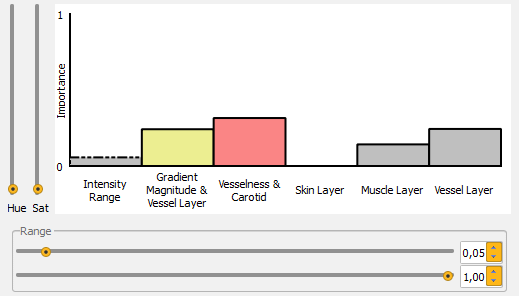
\includegraphics[width=0.75\linewidth]{figures/predicates/predicate_widget.png}
	\caption{Our \textbf{proposed widget} shows the predicate histogram and allows an easy and intuitive configuration of the point predicates for relevance-based rendering: The main area shows the distribution of predicate importances and enables easy manipulation using drag and drop. 
		Two sets of controls allow for further manipulation of the currently selected predicate: 
		The sliders on the left set up the color modulation; the controls on the bottom set up optional predicate parameters.}
	\label{fig:predicates:predicate_widget}
\end{figure}

The point predicates to apply are selected from the user or, alternatively, given by a workflow model later potentially learned specifically for the given anatomy and application. 
Each predicate has a small set of parameters, defining the predicate importance $\kappa$ and an optional color modulation $\delta$ having components hue $\delta^{(H)}$ and saturation $\delta^{(S)}$. 
Certain predicates may have further optional parameters defining where the predicate yields true (e.g. intensity range). 

We propose to combine predicate selection and configuration via the \emph{predicate histogram}, a single intuitive widget as shown in Figure \ref{fig:predicates:predicate_widget}. 
The heights of the bars directly represent the relative importance weighting of the predicates, while their fill color shows the color modulation. 
The user can manipulate the importance of each predicate with intuitive drag and drop interaction on the histogram bar and will directly see the results of his/her actions, as the predicate-based rendering is evaluated in real-time. 
In order to further reduce the parameter space without losing flexibility, the predicate histogram normalizes the sum of the predicates weights:
\begin{equation}
	\sum_j \kappa_j = 1.
	\label{eq:predicates:importance-normalization}
\end{equation}
Hence, increasing the importance of one predicate automatically decreases the importances of the other predicates and vice versa.
% \footnote{As this is a highly dynamic process, we encourage the reader to watch the video sequences in our supplementary material, showing the interactive manipulation of the predicate histogram and its real-time effects on the rendering.}. 

We place two additional sets of manipulators around the predicate histogram widget, which allow controlling additional parameters of the currently selected predicate: Two vertical sliders on the left allow the user to configure the color modulation in terms of hue and saturation. 
The resulting color is visualized in the predicate histogram as fill color of the corresponding bar. 
Furthermore, widgets to control feature specific predicate parameters (such as the range where the predicate yields true) are placed below the histogram in a horizontal layout. 

The predicate selection process is currently a fully manual task of explorative nature. 
However, we argue that achieving satisfying rendering results is significantly more intuitive and easier than with traditional 1D/2D transfer functions, since the parameter space of our point predicate technique is much more expressive due to its semantic nature and the whole process runs in real-time providing interactive feedback. 
Furthermore, the predicate histogram reduces the parameter space effectively in size through the normalization of predicate importances (cf. Equation \eqref{eq:predicates:importance-normalization}).


\subsection{Classification \& Compositing}
\label{sec:predicates:compositing}

For classification and compositing, our predicate-based ray caster evaluates the selected predicates on each input sample point $s$ to compute the sample importance $\kappa(s)$ and sample color modulation $\delta(s)$. 
As we wish the individual importances to contribute in an additive manner, we define $\kappa(s)$ as
\begin{equation}
	\label{eq:predicates:classification_importance_raw}
	\kappa(s) = \frac{\sum^n_{j=1} \chi_j(s) I(\kappa_j)}{\sum^n_{j=1} \chi_j(s)},
\end{equation}
where $I(\kappa_j)$ denotes the impact function for predicate $j$ and $\chi_j(s)$ the characteristic function for predicate $j$ (i.e. indicating whether $f_j(s)$ is true).
We would like the following two conditions to hold:
\begin{my_list_num}
	\item 
		A non-linear amplification of importance differences, meaning that $\kappa_i \sim \kappa_j \Rightarrow I(\kappa_i) \sim I(\kappa_j)$ but $\kappa_i < \kappa_j \Rightarrow I(\kappa_i) \ll I(\kappa_j)$.
		This allows for better usability since the user does not need to be pixel-perfect when assigning the same importance to multiple predicates. 
		This condition can be rewritten to 
		\begin{equation}
			\kappa_i - \kappa_j <  I(\kappa_i) - I(\kappa_j), 
		\end{equation}
		which holds for all differentiable $I$ with $I'(x) > 1$.
	
	\item
		In the case of all predicates having the same importance factor assigned, we wish $\kappa(s)$ to be always $1$:
		\begin{equation}
			\forall i,j : \kappa_i = \kappa_j   \quad \Rightarrow \quad   \forall s : \kappa(s) = 1.
		\end{equation}
\end{my_list_num}

Experimentally, we found $I(\kappa_j) := (n \cdot \kappa_j)^2$, where $n$ is the total number of predicates, to yield good results and satisfy both conditions. This gives us the following full definition (cf. Equation \eqref{eq:predicates:classification_importance_raw}):
\begin{equation}
	\kappa(s) = \frac{\sum^n_{j=1} \chi_j(s) \cdot (n \cdot \kappa_j)^2}{\sum^n_{j=1} \chi_j(s)}.
	\label{eq:predicates:classification_importance}
\end{equation}

It should be noted that one certainly can select very small $\kappa_i, \kappa_j$, so that $n \cdot \kappa_i < 0.5$ and $n \cdot \kappa_j < 0.5$ violate the first condition. However, in such cases there is at least one $\kappa_k$ with $n \cdot \kappa_k > 1$ due to Equation \eqref{eq:predicates:importance-normalization}. We argue that this effect is even desirable as predicate $k$ shall have the major impact on the visualization and we can neglect the importance difference between predicates $i$ and $j$.

In order to specify the optical properties of the sample $s$, we compute the sample color modulation in terms of hue $\delta^{(H)}(s)$ and saturation $\delta^{(S)}(s)$ in HSL color space.
The sample luminance as well as its opacity are set to the original ultrasound intensity.
This serves two goals:
It reduces the dimensionality of the parameter space, and even more importantly allows to retain the appearance of the original ultrasound data, which we see as an essential part of ultrasound visualization.
The color modulation is computed in an additive manner using the predicate contributions
\begin{equation}
	\omega_j(s) := \chi_j(s) \cdot (n \cdot \kappa_j)^2
\end{equation}
as weights.
The hue modulation is additionally weighted by the saturation modulation to avoid undesirable effects in cases where large hue shifts with small saturation modulations are combined with small hue shifts with large saturation modulations.
\begin{equation}
	\begin{aligned}
		\delta^{(S)}(s) 	&= \frac{1}{\sum_{j = 1}^n  \omega_j(s)} \cdot \sum_{j = 1}^n  \omega_j(s) \cdot \delta_j^{(S)}, \\
		\delta^{(H)}(s) 	&= \frac{1}{\sum_{j = 1}^n  \omega_j(s) \delta_j^{(S)}} \cdot \sum_{j = 1}^n  \omega_j(s) \delta_j^{(S)} \cdot \delta_j^{(H)}.
	\end{aligned}	
	\label{eq:predicates:classification_color}
\end{equation}

With sample importance, color and opacity set, the samples are fed into a focus and context compositing scheme.
While our proposed method should work with most relevance-based compositing techniques, we use use the one proposed by De Moura Pinto and Freitas \cite{Pinto10}, which has various desirable properties:
\begin{my_list_num}
	\item 
		Its well motivated front-to-back recurrence scheme formulation allows straightforward integration into standard ray casters.
	\item
		In the absence of importance values or with all samples being equally important, it resolves to the standard emission-absorption-based volume rendering integral.
	\item
		Its input parameters are clear and limited to a scalar importance value besides the standard optical properties of color and opacity. 
		We therefore map $\kappa(s)$ to $I_s$, $\delta(s)$ to $C_s$ and $I(s)$ to $\alpha_s$ as introduced in \cite{Pinto10}.
\end{my_list_num}	
The full recurrence scheme for compositing can be found in the Appendix.


\section*{Extensions}

Our technique integrates very well into the existing volume rendering pipeline. 
This is also valid for a variety of possible extensions that current state-of-the-art methods provide to facilitate standard transfer function-based classification, such as data driven techniques to generate transfer function presets, shape-based transfer functions, or image-driven transfer function setup where the user can manipulate the classification by direct interaction with the original image. 
Many of these works can be easily transferred to our predicate-based approach for direct volume rendering. 
As an example, we present how to integrate a scribble technique into our framework similar to the interface proposed by Tzeng et al. \cite{Tzeng03} and the stroke-based transfer function design by Ropinski et al. \cite{Ropinski08}. 

\begin{figure}[ht]
	\centering
	\subfloat[~Original Predicate Histogram]{
		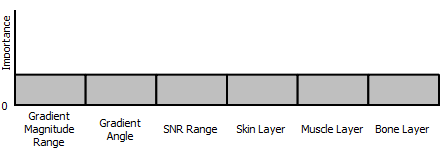
\includegraphics[width=0.75\linewidth]{figures/predicates/scribble_histogram_before.png}
		\label{fig:predicates:scribble:histogram-before}
	} \\%
	\subfloat[~Scribbles painted into cross-sectional slice views]{
		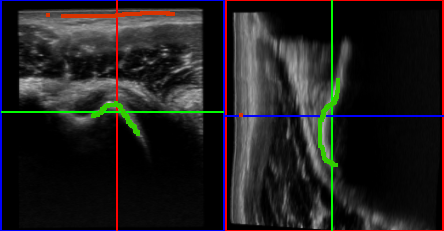
\includegraphics[width=0.75\linewidth]{figures/predicates/scribble.png}
		\label{fig:predicates:scribble:scribble}
	} \\%
	\subfloat[~Predicate Histogram After Applying Scribbles]{
		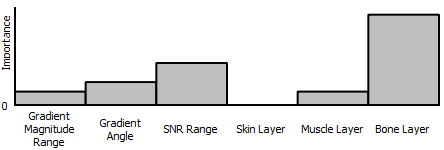
\includegraphics[width=0.75\linewidth]{figures/predicates/scribble_histogram_after.png}
		\label{fig:predicates:scribble:histogram-after}
	}
	\caption{
		\textbf{Illustration of scribble-based Predicate Histogram Setup}: \\
		(a) shows the original predicate histogram. 
		(b) By delineating image features to show (green scribble along bone structure) and image features to hide (red scribble in skin layer) in the cross-sectional MPRs, the user can configure the predicate histogram directly in the image domain. 
		(c) shows the updated predicate histogram after applying the scribbles.
	}
	\label{fig:predicates:scribble-fused}
\end{figure}
\begin{figure}[ht]
	\centering
	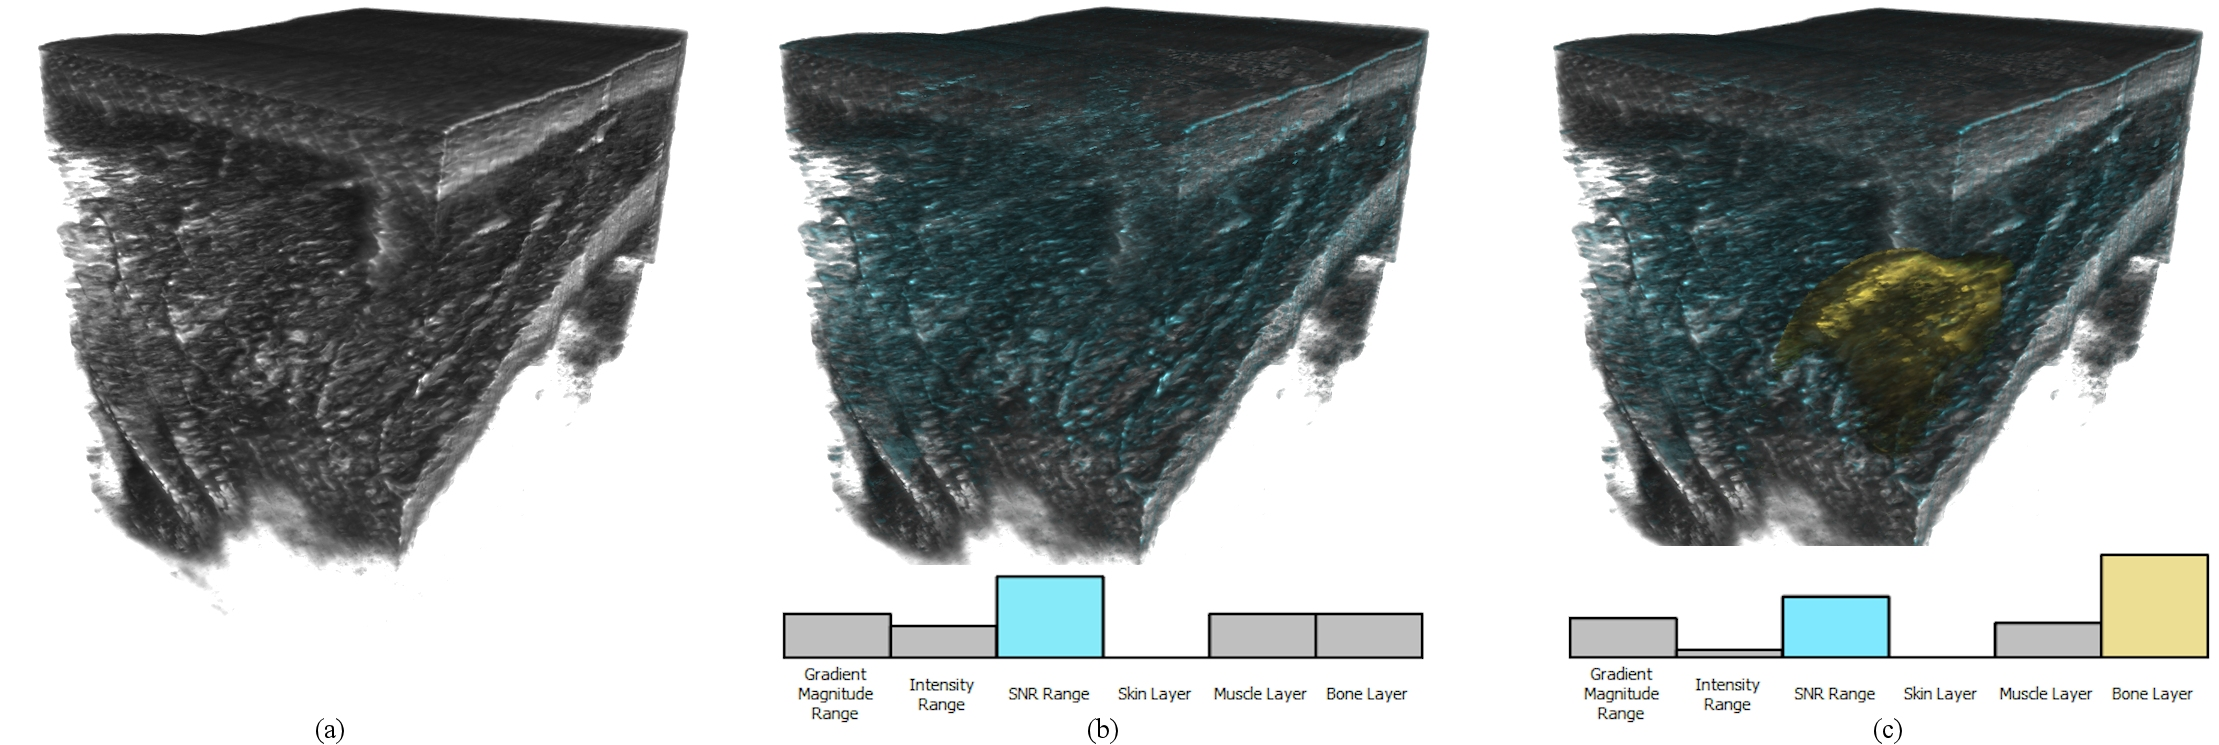
\includegraphics[width=0.95\linewidth]{figures/predicates/shoulder.jpg}
	\caption{
		Visualization results for the \textbf{shoulder data set} together with the used predicate histograms: 
		Compared to the standard transfer function-based visualization (a), (b) was generated by exploiting the SNR Range predicate to mark fibrous structures in the muscle layer. 
		The final rendering (c) additionally highlights the bone surface as focus region.
	}
	\label{fig:predicates:results-shoulder}
\end{figure}


\subsection{Scribble-based Predicate Histogram Setup}

While the predicate histogram widget already provides an intuitive metaphor to setup the predicate configuration, it still requires the user to perform an implicit mapping between the semantic meaning of each predicate and its corresponding features in the image. 
To further facilitate the predicate importance setup, we implemented a scribble technique that offers the user the possibility to directly interact with the ultrasound image by using a painting metaphor to mark focus and context regions in cross-sectional slice views of the volume as illustrated in Figure \ref{fig:predicates:scribble-fused}. 


The scribbles yield a set of positive samples that should be emphasized in the volume rendering and a set of negative samples that should be less prominent. 
Since emphasizing certain regions relates to increasing the importances of the corresponding predicates and since decreasing importances results in decreased visibility, we transform the scribbles into a modulation of the predicate importances $\kappa_i$. 

For each predicate $i$ we denote the number of positively labeled samples where the predicate yields true by $N^+_i$ and the number of negatively labeled samples where the predicate yields true by $N^-_i$. 
We compute an importance modulation vector $m$ as
\begin{equation}
	m_i = \frac{q \left(N^+_i - N^-_i \right)}{\sum_j N^+_j - N^-_j},
\end{equation}
where $q$ describes the percentage by which the current predicate histogram is altered through the scribbles, which we empirically set to $0.25$. 
In order to keep the predicate histogram in its normalized state (Equation \eqref{eq:predicates:importance-normalization}), we first normalize $m$ so that $\sum_j m_j = 0$ before we update each importance $\kappa_i$ by adding $m_i$. 

This approach can certainly be extended with more elaborate importance modulation or even automatic predicate parameter configuration. 
However, since this is beyond the scope of this paper we consider it as future work. 


\section*{Implementation}


We implemented our predicate-based ray casting technique entirely using OpenGL 4 and GLSL, so that apart from setting up the predicate logic, all evaluations and computations are performed on the GPU using a single fragment shader. 
Furthermore, our formulation is designed to seamlessly integrate into the standard direct volume rendering pipeline. 


\subsection{Predicate Selection \& Setup}
The client-side selection and setup is automatically transformed into shader code, for which we use a building block like system similar to the shader templates in \cite{Rautek08}. 
Every point predicate provides three blocks:
\begin{my_list_num}
	\item A \emph{GLSL header} defining uniform names for the predicate parameters and further optional definitions. 
	\item A \emph{closed GLSL expression} defining how to evaluate the predicate with respect to the input data. 
	\item A \emph{function to setup the shader}, which is called by the renderer (prior to rendering) and assigns the parameter values to the corresponding uniforms. 
\end{my_list_num}
The classification scheme from Equations \eqref{eq:predicates:classification_importance} and \eqref{eq:predicates:classification_color} is transformed into a single GLSL function combining the evaluation expressions and yielding the final sample intensity and color modulation. 
Together with the predicates' GLSL headers, the predicate evaluation function is injected into the renderers fragment shader. 
Meta predicates are easily implemented using a composite pattern. 

Potentially expensive recompilation of the shader has to be performed only when the set of selected point predicates changes, as this is the single event changing the definition of uniform variables and predicate expressions. 
Subsequent rendering setup by configuring the predicates' importance factors, color modulations, and optional parameters is entirely implemented by updating the uniform values, which is even less overhead than an update of the transfer function texture as performed by traditional transfer function-based renderers. 

To implement the proposed scribble technique, we need to encode for each pixel which predicates yield true. 
This is easily done by generating a 3D volume where each voxel encodes the results of the predicates' characteristic functions in a bit mask. 



\subsection{Integration into the Standard DVR Pipeline}

Integrating our predicate-based classification and compositing into a standard GLSL ray caster is straightforward and needs only minimal changes in the shader code: Instead of a texture lookup on the transfer function, the shader gathers all necessary input data for the predicates and calls the predicate evaluation function yielding final sample importance and color modulation. 
The color modulation is then applied to sample intensity in HSL space, yielding the sample color value and opacity. 
Together with the sample importance they are directly fed into the compositing scheme as defined in \cite{Pinto10}. 


\section*{Results}
\label{sec:predicates:results}

\begin{figure}[ht]
	\centering
	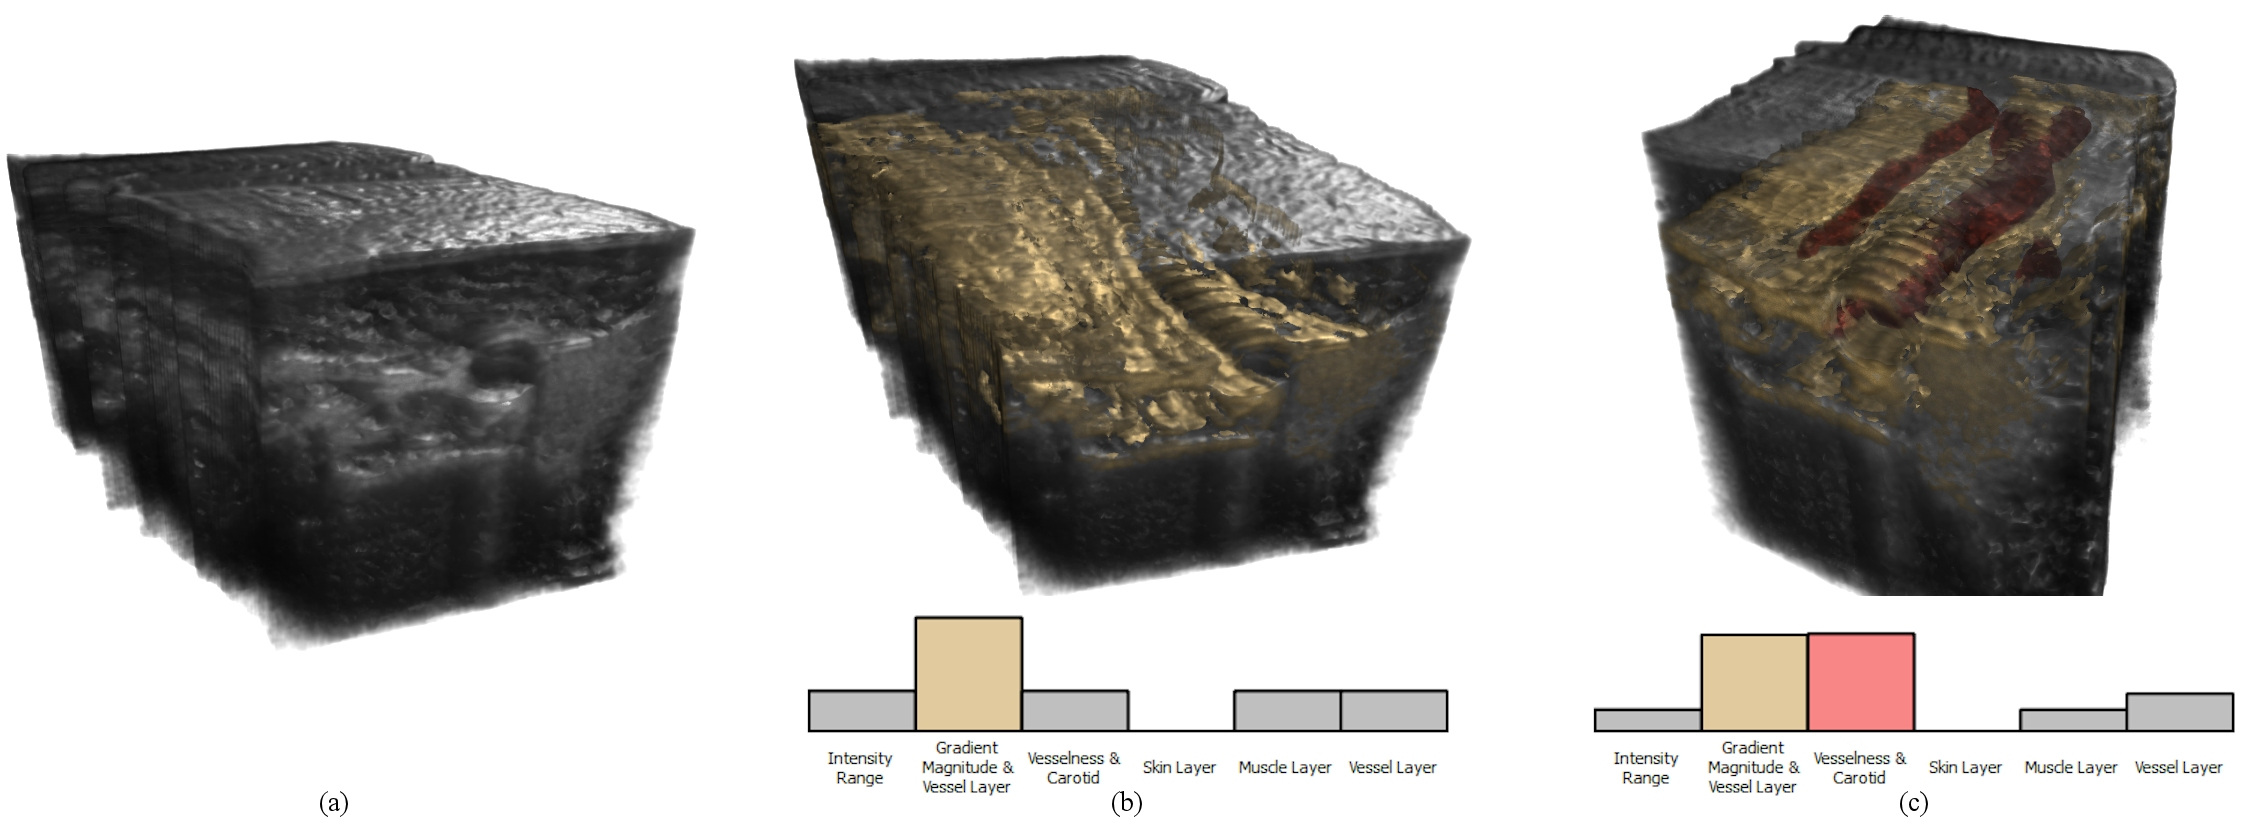
\includegraphics[width=0.95\linewidth]{figures/predicates/carotid2.jpg}
	\caption{
		Visualization results for the second \textbf{carotid artery data set} together with the used predicate histograms: 
		Compared to the standard transfer function-based visualization (a), the predicate setup in (b) removes the skin layer and highlights vascular structures. 
		The vesselness predicate in (c) allows to further show the vessel path (the bifurcation is only partly present in this data set and thus can not be seen).
	}
	\label{fig:predicates:results-carotid2}
\end{figure}
\begin{figure}[ht]
	\centering
	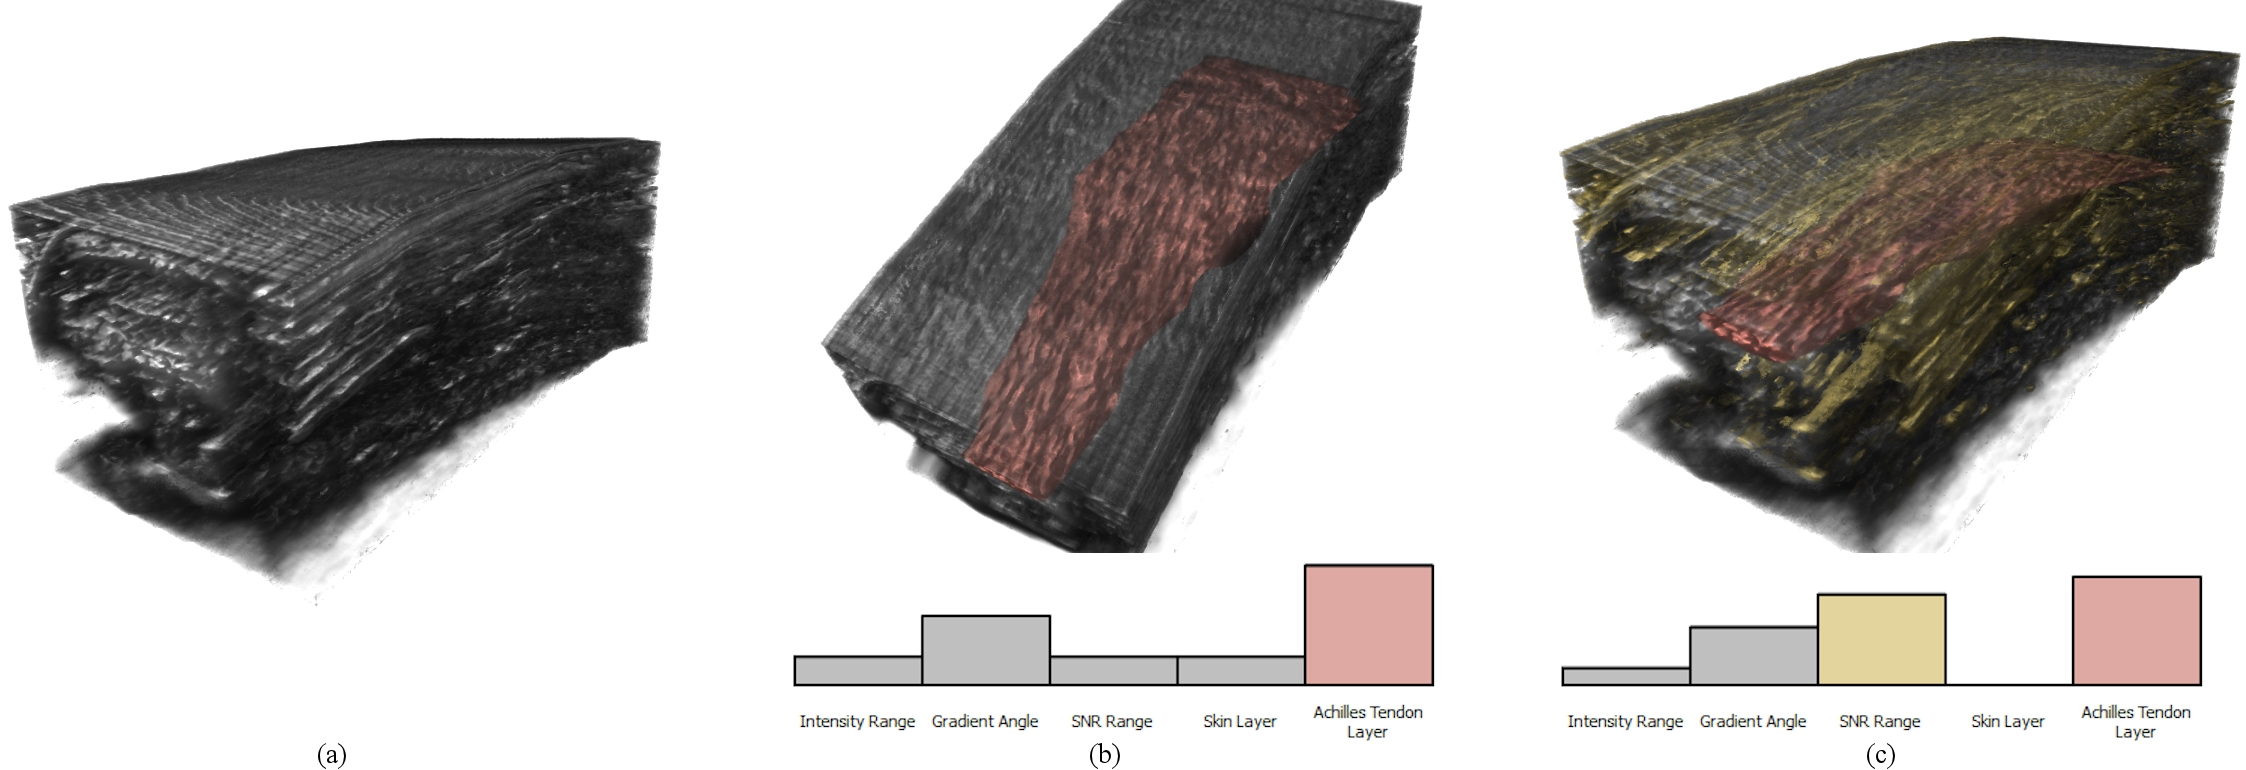
\includegraphics[width=0.95\linewidth]{figures/predicates/achilles.jpg}
	\caption{
		Visualization results for the \textbf{achilles tendon data set} together with the used predicate histograms: 
		Compared to the standard transfer function-based visualization (a), (b) highlights the target anatomy (achilles tendon) through the gradient angle predicate and the corresponding label predicate. 
		(c) Shows the final rendering with highlighted fibrous muscle structures as context information using the SNR range predicate.
	}
	\label{fig:predicates:results-achilles}
\end{figure}

For evaluation we acquired ultrasound sweeps of three distinct anatomies (shoulder, carotid artery, and achilles tendon) using an ACUSON S2000\texttrademark~ultrasound machine equipped with an Acuson 9L4 linear transducer and electromagnetic tracking hardware. 
These sweeps were reconstructed using an advanced backward compounding algorithm exploiting frame orientation information to yield high quality volumes. 
Further details on this algorithm can be found in \cite{SzB14}.
The resulting volumes have a resolution of $512^3$ voxels for the shoulder data set and of $384^3$ voxels for the carotid and the achilles tendon data set.
% \footnote{Download links to our data sets can be found in the supplementary material.}
% These sweeps were reconstructed using an advanced backward compounding algorithm similar to the one proposed by Wein et al. \cite{Wein06} yielding 3D volumes  of $512^3$ voxels for the shoulder data set and of $384^3$ voxels for the carotid and the achilles tendon data set\footnote{Download links to our data sets can be found in the supplementary material.}.


After discussions with clinicians we identified clinically relevant features for each data set: For the shoulder data set, the clinicians were interested in seeing the bone surface in context with the muscle layer. 
Figure \ref{fig:predicates:results-shoulder} shows possible visualization results of our technique in conjunction with the predicate histogram used. 
3D Visualization of carotid ultrasound specifically needs to show the path of the carotid artery and its bifurcation in a spatial context, as shown in Figures 1 and \ref{fig:predicates:results-carotid2}. 
Finally, for the achilles tendon acquisition, the clinicians need to see the tendon in its whole shape in order to identify possible tears or other lesions. 
Figure \ref{fig:predicates:results-achilles} shows the results of our approach. 


To support our predicate-based approach to classification, we performed a manual segmentation on the data sets partitioning the ultrasound volumes into semantic layers of anatomy such as skin, muscle and bone (cf. Section \ref{sec:predicates:methods:predicates} on label predicate).
% Please note that {(semi-)} automatic segmentation is beyond the scope of our work but can later be integrated into the predicate concept in a straight-forward fashion. 

\begin{figure}[ht]
	\centering
	\subfloat[~Carotid ultrasound data set 1]{
		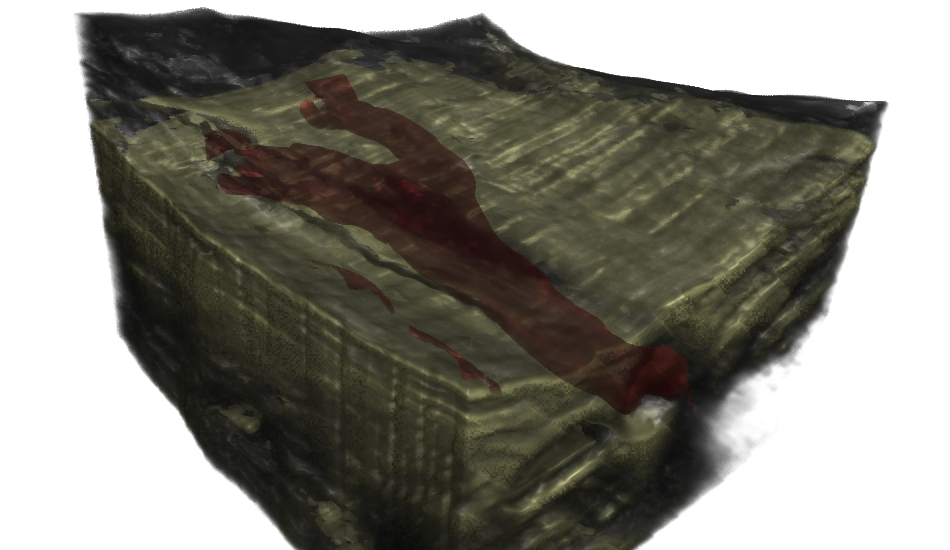
\includegraphics[width=0.75\linewidth]{figures/predicates/comp_1.jpg}
	} \\%
	\subfloat[~Used predicate histogram]{
		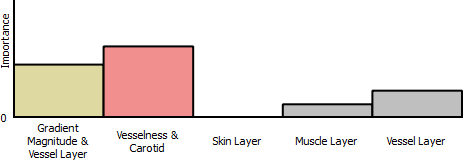
\includegraphics[width=0.75\linewidth]{figures/predicates/comp_histogram.png}
	} \\%
	\subfloat[~Carotid ultrasound data set 2]{
		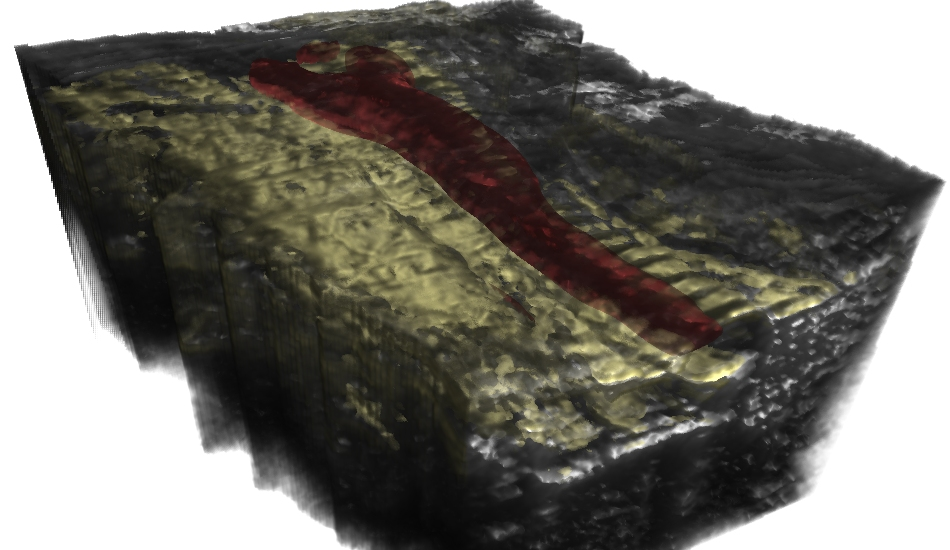
\includegraphics[width=0.75\linewidth]{figures/predicates/comp_2.jpg}
	}
	\caption{
		Results suggest a \textbf{transferability of predicate histograms} between different data sets of the same anatomy: 
		(a) A visualization for carotid data set 1 was created using the predicate histogram (b).
		This was then applied as preset to carotid data set 2 yielding a very viable visualization (c).
	}
	\label{fig:predicates:histogram-transferability}
\end{figure}

To evaluate the transferability of the predicate histogram setup, we applied the same configuration to both our carotid ultrasound data sets. 
As depicted in Figure \ref{fig:predicates:histogram-transferability}, a single predicate histogram was able to create a proper visualization for both data sets. 
This suggests that our formulation allows to reuse a predicate histogram, which was created for a specific data set, for a different data set of the same anatomy as valid preset, so that the user does not need to start the exploration and tuning from scratch.

All results presented in this work were acquired in interactive sessions with a nVidia GeForce 670 GTX GPU. 
While implementing a performance-optimized rendering was not our main goal, our implementation is still capable of generating sufficient frame rates for interactive renderings as shown in Table 1. 
The decreased performance in comparison to standard 1D transfer function-based direct volume rendering is mainly because the illustrative focus-and-context rendering does no longer allow for early ray termination. 

\begin{table}[th]
	\centering
	\begin{tabu} to 0.9\linewidth {>{\bfseries\centering}m{50mm} C C}
		\toprule
		                          & \bfseries Achilles Tendon & \bfseries Shoulder \\
		                          & ($384^3$ voxels)          & ($512^3$ voxels)   \\
		\midrule
		Standard 1D TF-based      & $102.3$ fps               & $30.4$ fps         \\
		Predicate-based Rendering & $38.9$ fps                & $15.7$ fps         \\
		\bottomrule
	\end{tabu}
	\label{tbl:predicates:fps}
	\caption{Frame rates of our predicate-based approach compared to standard 1D transfer function-based direct volume rendering for different data sets on a GeForce 670 GTX, viewport size $800$x$600$.}
\end{table}


\section*{Discussion}

In the previous section, we compared our rendering results only to standard direct volume rendering with a 1D grayscale transfer function, which may raise the question how our technique compares to other related visualization techniques referenced in Section \ref{sec:predicates:related_work}. 
The main issue is that most of these techniques are not applicable to ultrasound data.
Ultrasound intensities are of highly context-sensitive nature (cf. Section \ref{sec:predicates:related_work:us}) so that transfer functions solely relying on local information, such as intensity and gradient, neither improve the visual outcome nor are a suitable domain for defining color.
Since our results rely to some extent on segmentation output, our approach can be seen as specialization of multi-volume rendering techniques, which could yield similar results.
However, we would like to stress that the focus of our work is the full integration of a large variety of classification techniques into a single consistent formulation in combination with an intuitive user interface that allows for highly interactive exploration of the data.


One side effect of relevance-based rendering is the limited depth perception, in particular in still images. 
It is an inherent property of this approach that features, which would usually be occluded, pop out if they are assigned with a higher importance factor than features in the front. 
The correct depth perception can however still be perceived for instance through motion parallax in dynamic scenes as shown in our video in the supplementary material.
Furthermore, the used compositing scheme \cite{Pinto10} ensures a correct depth ordering in case of uniform importances so that the depth perception of the individual features themselves remains intact.


A very important aspect is the intuitiveness of our predicate histogram based on the semantic nature of the predicates.
Therefore, it is essential to provide the predicates and their settings with easily comprehendable naming.
Since all the user needs to do is deciding whether he/she wants to see more or less of a certain feature and adjust the corresponding bar in the predicate histogram accordingly, this can also be considered as an implicit parameter space reduction

It should be noted that the focus of this paper is the introduction of the predicate concept and the predicate histogram, as well as the demonstration its potential on selected examples. 
An exhaustive study regarding the selection of suitable features for defining predicates is beyond the scope of this paper, as are techniques for automatic segmentation of specific anatomies. 
For a detailed overview on suitable segmentation techniques, we refer the interested reader to the book of Szeliski \cite{Szeliski10} or the survey paper of Heimann and Meinzer \cite{Heimann09}. 
Due to our generic formulation, segmentation results obtained by such techniques or even the techniques themselves can be easily transferred into predicates and integrated into our visualization concept.

\section*{Conclusion}
In this work, we introduced a novel consistent formulation for predicate-based classification of volumetric image data. 
It does not only allow for integration of both local and global image information and even anatomical models, but also naturally extends to illustrative focus-and-context visualization. 
While our technique does not make any a-priori assumptions on the type of input data or its spatial representation, it was designed for the specific application of direct volume visualization to 3D ultrasound volumes, for which it yields superior results in terms of occlusion and distinctly exposing selected image features than traditional global transfer function-based visualization. 

To complement our approach, we additionally proposed the predicate histogram as an effective means for reducing the potentially high dimensionality of the predicate configuration domain. 

It provides the user with an intuitive interface showing an overview over the parameter space, as well as with interaction metaphors to interactively manipulate the visualization result in real-time. 
Especially in combination with the implemented scribble technique, the predicate histogram can be modified by direct interaction with the rendered ultrasound image. 
Thus, we obtain an intuitive workflow, which allows also non-expert users to obtain insightful visualizations. 
The whole framework is designed to seamlessly integrate in the standard volume rendering pipeline without significantly increasing the computational burden and thus allowing for a real-time interaction with the system. 


While directly integrating adequate segmentation technique into our predicate formulation might be one aspect of future work, other aspects are the application of our technique to other imaging modalities and multi-modal data sets.
We imagine the predicate domain to be well suited for machine learning approaches, which could generate application-specific workflow models to automatically provide predicate histogram presets. 


\section*{APPENDIX}
\label{sec:predicates:appendix}
\newcommand{\vis}{\text{vis}(\kappa(s), \kappa_i)}

The detailed recurrence scheme for the relevance-based compositing of our technique is as follows. The equations are the same as in \cite{Pinto10} but adapted to our naming conventions.

Let $\kappa(s)$ be the computed sample importance, $C(s)$ be the sample color and $\alpha(s)$ be the sample opacity as we defined in Section \ref{sec:predicates:compositing}. 
Then we define the visibility factor $\vis$ of the current sample $\kappa(s)$ compared to the accumulated importance $\kappa_i$ as
\begin{equation}
	\vis		=		1 - \exp (\kappa_i \kappa(s)),
\end{equation}
as well as the modulation factor $m$ as
\begin{equation}
	m  = 
	\begin{cases}
		1							&		\kappa(s) \leq \kappa_i, \\
		1							&		1-\alpha_i \geq \vis, \\
		\frac{1-\vis}{\alpha_i}		& 	\text{else}.
	\end{cases}
\end{equation}
The incremental front-to-back compositing scheme is defined by:
\begin{equation}
	\begin{aligned}
		C'_{i+1}				&=		m C_i + (1 - m \alpha_i) C(s), \\
		\alpha'_{i+1}			&=		m\alpha_i (1 - \alpha(s)) + \alpha(s), \\
		\alpha_{i+1}			&=		\alpha_i (1 - \alpha(s)) + \alpha(s), \\
		C_{i+1}					&=		
		\begin{cases}
			0                                           & \alpha'_{i+1} = 0, \\
			\frac{\alpha_{i+1} C'_{i+1}}{\alpha'_{i+1}} & \text{else},
		\end{cases}\\
		\kappa_{i+1}			&=		\max(\kappa_i, \ \ln(\alpha(s) + (1 - \alpha(s)) \exp(\kappa_i - \kappa(s))) + \kappa(s)).
	\end{aligned}
\end{equation}

\cleardoublepage

\section{Challenges in 3D Ultrasound Visualization}

\section{Point Predicates as Generic Concept for Classification}

\section{The Predicate Histogram}

\section{Predicate-based 3D Ultrasound Visualization}

\section{Scribble-based Predicate Histogram Setup}

\section{Results and Evaluation}
